%     - Zobrazování dat - Grafana vs Vue grafy
%         - screenshot(y), jak to vypadá

\section{Zobrazování dat}
\label{sec:implementation:visualization}

\todo{Doplnit odkaz na sekci návrhu vizualizace a krátký úvodní odstavec shrnující, co tato sekce popisuje (implementaci vizualizací navržených v \sectionref{sec:design:visualization}).}

Hlavní vizualizací je zobrazení vývoje stavu \PR v~čase (\textit{PR State Over Time}), zachycené na \customref{Obrázku}{fig:visualization:pr_state_over_time}. Uživatel zvolí repozitář, stav \PR, kotevní datum a~počet zpětně zobrazovaných dní. Na základě těchto parametrů je zavolán endpoint \code{/api/pr/prs-in-state-over-time}, který vrátí denní počty \PR v~daném stavu. Nad grafem jsou zobrazeny souhrnné statistiky za zvolené období: aktuální hodnota, průměr, minimum, maximum a~trend (rozdíl mezi aktuální hodnotou a~průměrem).

\begin{figure}[H]
  \centering
  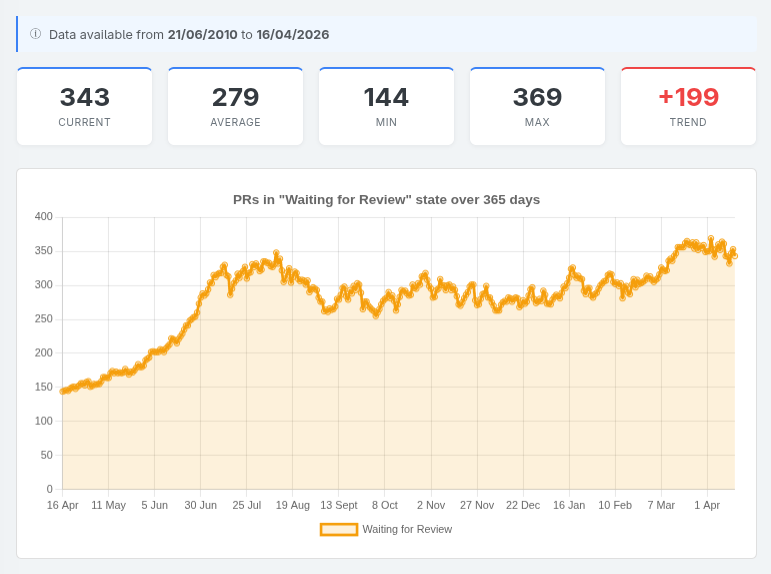
\includegraphics[width=0.8\textwidth]{figures/visualization/pr_state_over_time.png}
  \caption{Zobrazení vývoje počtu \PR ve stavu \uv{Waiting for Review} za posledních 365 dní}
  \label{fig:visualization:pr_state_over_time}
\end{figure}

Druhým pohledem je souhrn všech stavů naráz (\textit{All States Combined}), zobrazený na \customref{Obrázcích}{fig:visualization:all_states_full} a~\ref{fig:visualization:all_states_filtered}. V~tomto režimu jsou na jediném grafu vyneseny křivky pro všechny stavy současně. Uživatel může jednotlivé křivky interaktivně skrývat a~zobrazovat kliknutím na jejich popisek v~legendě. Tato funkce je zvláště užitečná při porovnání stavů s~výrazně odlišnými hodnotami na ose $y$ — například skrytím monotónně rostoucích křivek \textit{Open}, \textit{Closed} a~\textit{Merged} se odhalí detailnější průběh stavů \textit{Waiting for Review}, \textit{Waiting for Author} a~\textit{Waiting for Bors}, jak ukazuje \customref{Obrázek}{fig:visualization:all_states_filtered}.

\begin{figure}[H]
  \centering
  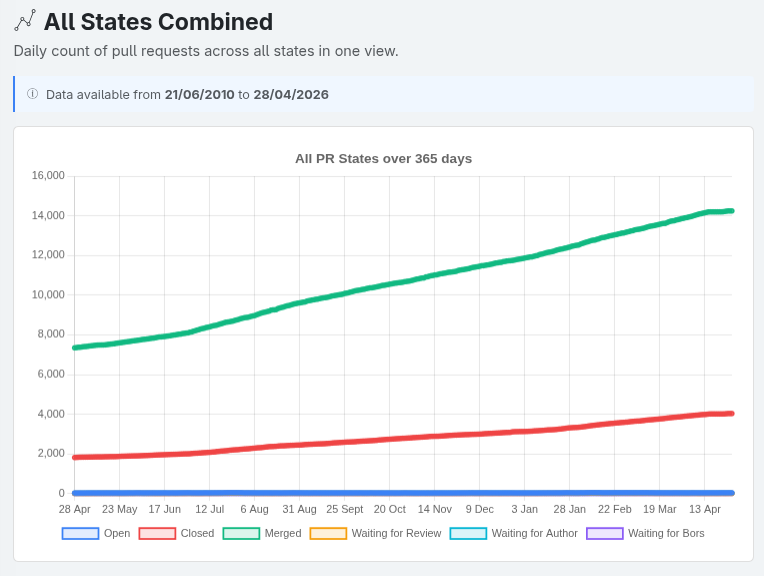
\includegraphics[width=0.8\textwidth]{figures/visualization/all_states_combined.png}
  \caption{Souhrn všech stavů \PR za posledních 365 dní — plné zobrazení}
  \label{fig:visualization:all_states_full}
\end{figure}

\begin{figure}[H]
  \centering
  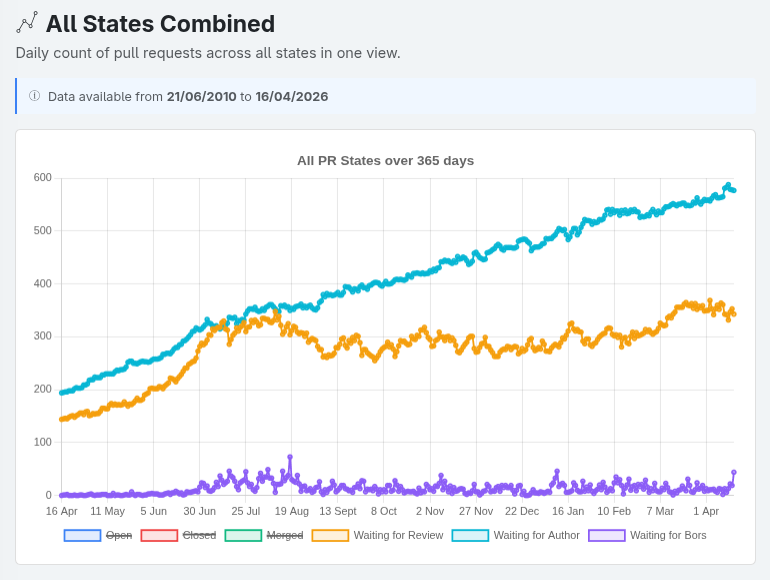
\includegraphics[width=0.8\textwidth]{figures/visualization/all_states_filtered.png}
  \caption{Souhrn stavů \PR po skrytí monotónně rostoucích křivek — detail \PR čekajících na akci}
  \label{fig:visualization:all_states_filtered}
\end{figure}

Další vizualizací jsou soubory upravené členy daného týmu v~zadaném časovém okně, dostupné přes endpoint \code{/api/pr/files-modified-by-team}. Uživatel zadá název repozitáře, název týmu, kotevní datum a~počet dní pro zpětný pohled. Výsledkem je seznam souborů seřazený sestupně podle počtu úprav. Klíčovým parametrem je \code{group\_level}, který určuje způsob seskupení výsledků:

\begin{itemize}
  \item \code{none} (výchozí) — plochý seznam jednotlivých souborů s~počtem úprav,
  \item číslo (např. \code{1}, \code{2}) — seskupení do adresářové hierarchie do zadané hloubky; hodnota \code{1} seskupí soubory do složek nejvyšší úrovně (\code{src/}, \code{library/} apod.), hodnota \code{2} dále rozdělí výsledky na podadresáře (\code{src/doc/}, \code{library/core/} apod.),
  \item \code{all} — úplná adresářová hierarchie rekurzivně až na úroveň jednotlivých souborů.
\end{itemize}

Možnost plochého seznamu je zahrnuta z~důvodu, že v~takovém případě není nutná transformace dat z~databáze do stromové struktury. Sploštování stromové struktury na straně klienta by navíc bylo pomalejší než přímé zobrazení dat ve správném formátu.

Díky parametru \code{group\_level} lze snadno identifikovat, na které části projektu se daný tým v~daném období zaměřoval, aniž by bylo nutné procházet stovky záznamů v~plochém seznamu.

Výchozí zobrazení bez seskupení (\code{group\_level=none}) je zachyceno na \customref{Obrázku}{fig:visualization:files_list}. Výsledky jsou prezentovány jako horizontální sloupcový graf doplněný tabulkou se seřazeným seznamem souborů a~jejich počty úprav.

\begin{figure}[H]
  \centering
  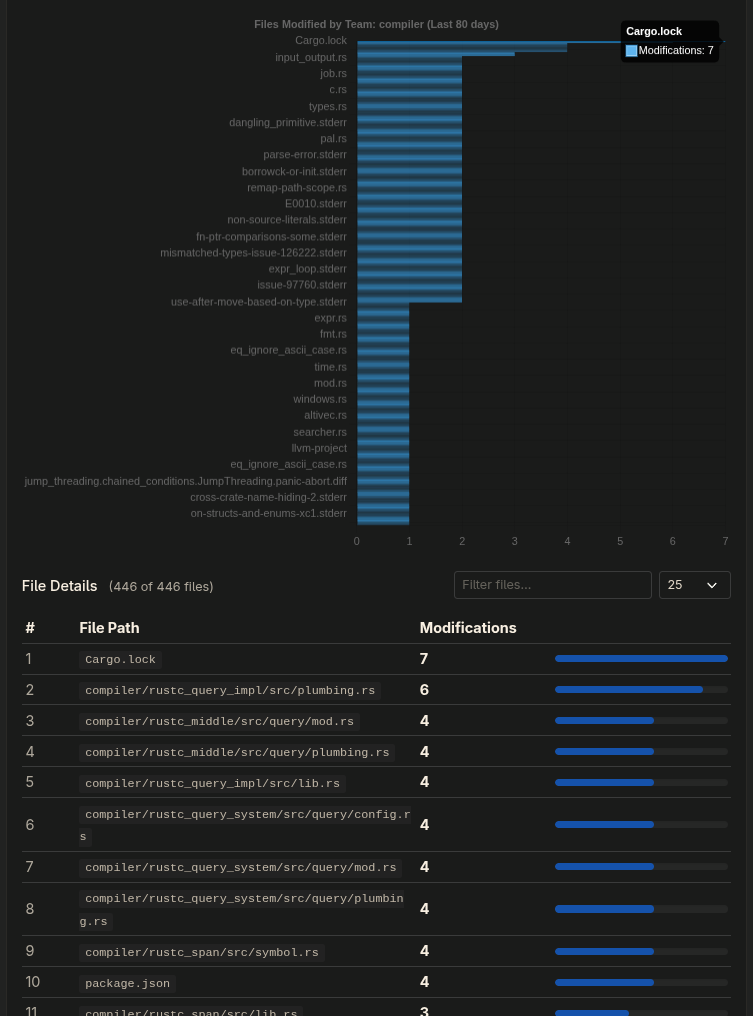
\includegraphics[width=0.9\textwidth]{figures/visualization/files_edited_team_list.png}
  \caption[Soubory upravené týmem — plochý seznam]{Soubory upravené týmem \uv{compiler} za posledních 80 dní — plochý seznam (\code{group\_level=none})}
  \label{fig:visualization:files_list}
\end{figure}

Při seskupení s~parametrem \code{group\_level=all} je výsledná stromová struktura vizualizována jako treemap, viz \customref{Obrázek}{fig:visualization:files_tree}. Plocha každého bloku odpovídá relativnímu počtu úprav dané složky nebo souboru vůči ostatním. Kliknutím na blok lze přejít do příslušné podúrovně hierarchie. Díky tomu lze na první pohled odhalit, které části repozitáře jsou daným týmem nejaktivněji upravovány.

\begin{figure}[H]
  \centering
  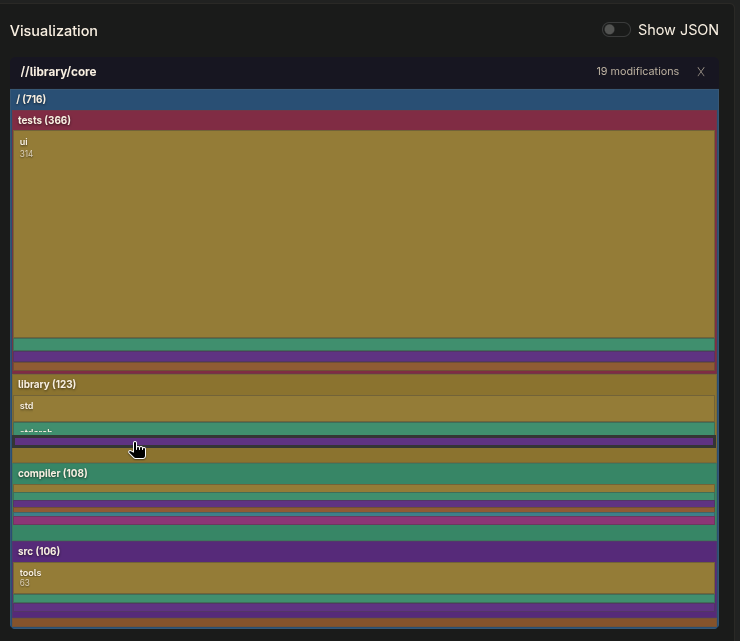
\includegraphics[width=0.9\textwidth]{figures/visualization/files_edited_team_tree.png}
  \caption[Soubory upravené týmem — treemap]{Soubory upravené týmem — hierarchická vizualizace (treemap, \code{group\_level=all})}
  \label{fig:visualization:files_tree}
\end{figure}

Frontend navíc umožňuje přepnout do režimu zobrazení surové \JSON odpovědi z~\API, jak ukazuje \customref{Obrázek}{fig:visualization:files_json}. Tento pohled slouží zejména pro ladění a~ověřování správnosti vrácené stromové struktury.

\begin{figure}[H]
  \centering
  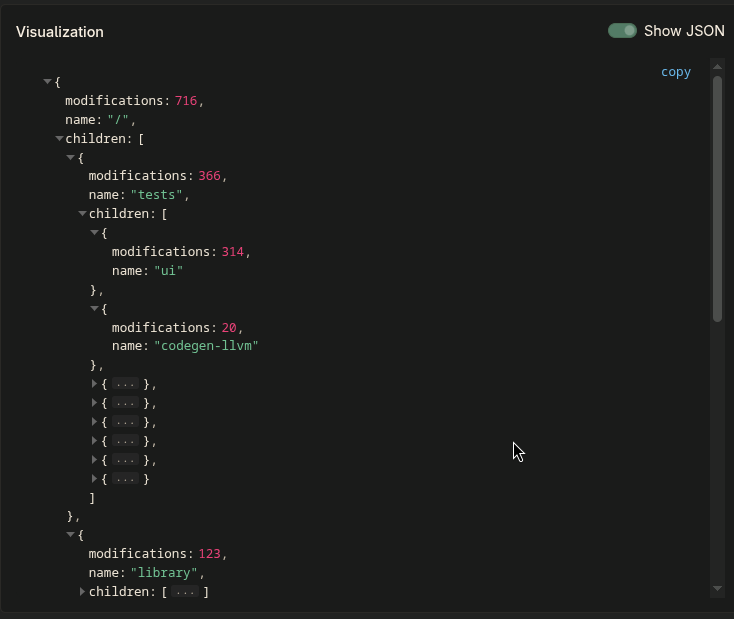
\includegraphics[width=0.9\textwidth]{figures/visualization/files_edited_team_json.png}
  \caption[Surová \JSON struktura stromové hierarchie souborů]{Surová \JSON struktura stromové hierarchie souborů vrácená \API}
  \label{fig:visualization:files_json}
\end{figure}